\documentclass[10pt,a4j,twocolumn]{jsarticle}

\usepackage[dvipdfmx]{graphicx}

\setlength{\textheight}{275mm}
\headheight 5mm
\topmargin -30mm
\textwidth 185mm
\oddsidemargin -15mm
\evensidemargin -15mm
\pagestyle{empty}
\begin{document}
\title{MathJaxを用いたhikiでの数式表示の簡易化}
\author{関西学院大学 情報科学科 西谷研究室 2535 那須比呂貴}
\date{}
\maketitle
\section{目的}
西谷研で行われる数値計算のプログラム開発において,数式を多用した文書作成が必須である.
また,文書提供にはwebベースのhikiにより管理がなされている.
しかし,hikiにおいて数式を表示するために使われてきたMathMLへの変換ソフトの
メンテナンスが近年なされておらず,これらのシステムを見なおす必要が出てきた.
本研究の目的は,
MathJaxを用いることにより,hiki上で数式をきれいにかつ容易に表示させる
システムを開発することである.

\section{既存システムの評価}
\subsection{hikiについて}
サイト構築や更新を手軽にできるWikiクローンの1つであるhikiを利用している.
Wikiとの違いはコードがRubyで記述されていることである.
hikiは,hikidocというライブラリを使うことで,hiki文法で書かれたテキストをHTMLに変換している.
hikiには下記の特徴がある.
\begin{enumerate}
\item プラグインによる機能拡張
\item アクセス制限の管理が容易
\item ページの追加,編集がしやすい
\item 出力するHTMLを柔軟に変更可能
\item システムのプロトタイプを容易に作成できる
\end{enumerate}
\subsection{MathJaxについて}
ブラウザーで数式を表示するには,画像を使うか,MathMLを使うのが通常の手法である.
画像を使う典型例としてlatex2hikiがある.
ところが,画像の管理や,拡大,印刷した時のクオリティーの低さが問題である.
一方,MathMLはコンピュータによる数式の意味認識において有利となるよう設計されたものであり,
人間がMathMLを直接書いたり編集したりすることは意図していない.
したがって,人間が書きやすいlatexから自動変換が提供されている.
hikiでは,Ruby 用ライブラリであるmathml.rbを利用している\cite{hiraku}.
しかし,MathMLが標準で提供されるブラウザーはFirefoxに限られており,一般ユーザがIEで利用するには特殊なadd onをinstallする必要がある.

近年開発が始まった,MathJaxはこのような欠点を克服して,
\begin{enumerate}
\item MathJaxはLaTeXの数学環境コマンドを再現できる.
\item MathML未対応のブラウザでも表示できるようにすることができ,ユーザが事前準備をしなくても良い.
\item 画像化しないので拡大したり,高解像度で印刷しても鮮明である.
\item MathJaxをウェブページコンテンツと一緒にダウンロードし,ページ中の数式マークアップを走査し,数式を組版することができる.
\end{enumerate}
以上の特徴より,本研究ではMathJaxを用いることが適当と考えた.

\section{hiki上でのMathJaxの導入手順}
\subsection{hikiとMathJaxを連携させ,hikiで入力した内容をMathJax化させる}
hikiでのmathjax表示は次のようにして実現できる.
\begin{itemize}
\item JavaScriptをdirectory内に用意
\item hikiのlayoutのひな形template/layourt.htmlの一部を変更
\end{itemize}
次の通り,latex形式で書き込んだhiki文書が
\begin{quote}\begin{verbatim}
$f_x$
$$f(\rho) =\sqrt{\rho}=\sqrt {\sum_j h^2 }$$
\end{verbatim}\end{quote}
hikiのシステムによってweb上では次のように表示される.


\begin{figure}[h]
  \centering
  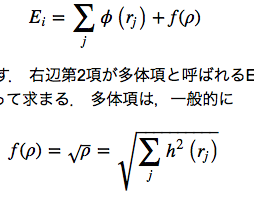
\includegraphics[width=5cm]{Math_test3.png}
  \caption{web上の内容}
\end{figure}

\subsection{今後の課題}
hikiではプラグインで提供されるのが標準である.
したがって,前述のような手作業による改変は標準的なinstallとして望ましくない.
そこで前述の作業を自動化するpluginを実装する.

\section{参照文献}\begin{enumerate}
\item\verb|mathml, ひらく工房(http://www.hiraku.ro/?mathml.rb)|, 黒田 ひらく, 2016/8/31アクセス.
\end{enumerate}
\end{document}
